\newpage
\section{Auswertung}
\label{sec:Auswertung}

Die in \autoref{sec:Auswertung} gezeigten Grafiken und Ausgleichsrechnungen sind mithilfe der Python-Bibliotheken Matplotlib \cite{matplotlib}, Scipy \cite{scipy} und Numpy \cite{numpy}
erstellt worden.

\subsection{Überprüfung der Bragg-Bedingung}

Wie in der Durchführung beschrieben wird ein fester Kristallwinkel von $\Theta = 14°$
eingestellt. 
\begin{figure}[H]
  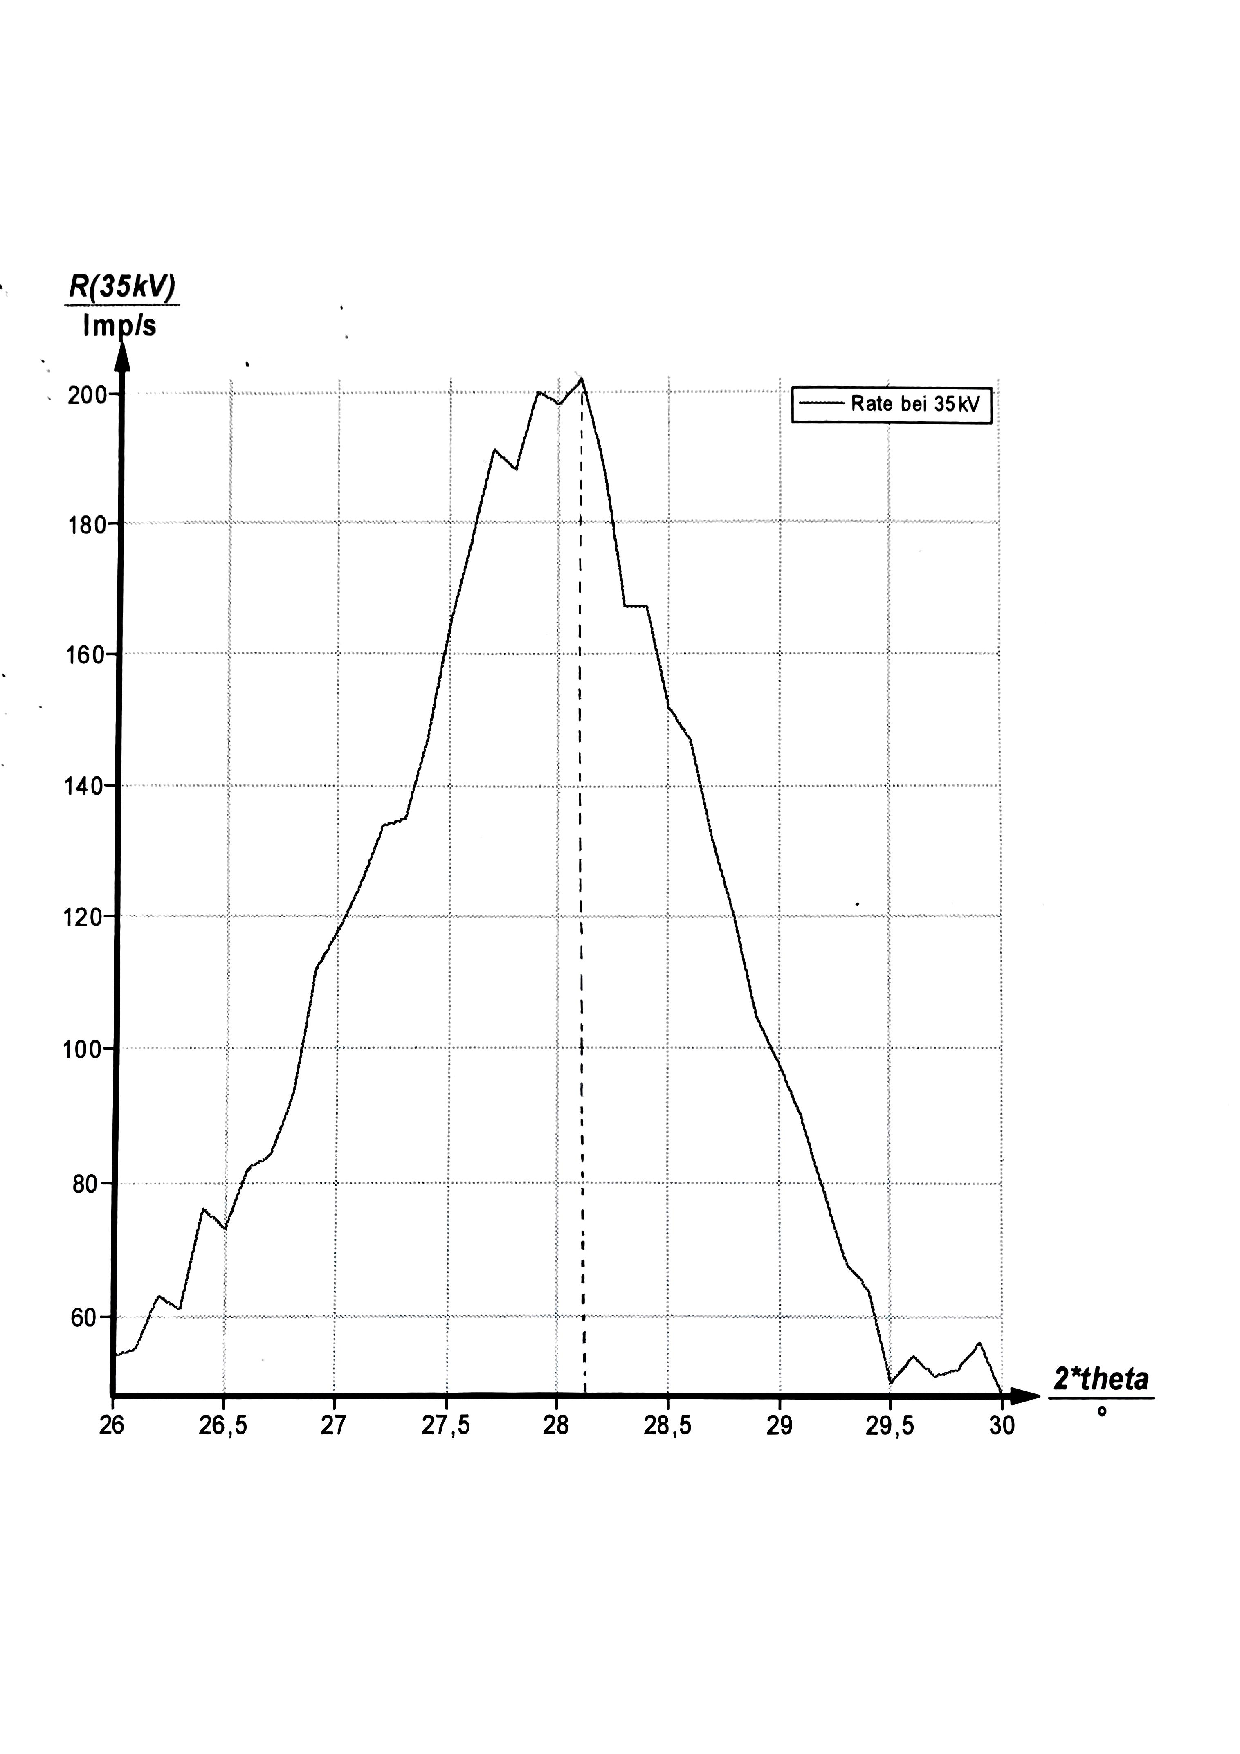
\includegraphics[width=\linewidth, height=14cm]{build/braggbedingung.pdf}
  \caption{Messergebnisse der ersten Versuchsreihe und erwartetes Maximum.}
  \label{fig:braggbedingung}
\end{figure}
Das Maximum der Kurve lässt sich aus \autoref{fig:braggbedingung} bei
\begin{equation*}
  \Theta_{max} = \SI{28.1}{°}
\end{equation*}
ablesen und beträgt
\begin{equation*}
  R_{max} = \SI{203}{Imp/s}.
\end{equation*}

\subsection{Das Emissionsspektrum einer Cu-Röntgenröhre}
\begin{figure}[H]
  \includegraphics[width=\linewidth, height=14cm]{build/bremsberg.pdf}
  \caption{Emissionsspektrum einer Cu-Röntgenröhre.}
  \label{fig:spektrum}
\end{figure}

In \autoref{fig:spektrum} ist der Bremsberg gekennzeichnet. Die K-Linien lassen sich in \autoref{fig:detail} bei 
\begin{align*}
  \Theta_{\beta} &= \SI{20.2}{°} \\
  \text{und }\Theta_{\alpha} &= \SI{22.5}{°}
\end{align*}
ablesen.
\begin{figure}[H]
  \includegraphics[width=\linewidth, height=14cm]{build/detail.pdf}
  \caption{Detailspektrum der $K_{\alpha}-$ und $K_{\beta}-$Linie.}
  \label{fig:detail}
\end{figure}
Mit \autoref{} und \autoref{} ergibt sich für die frei werdende Energie
\begin{align*}
  E_{\alpha} &= \SI{8044}{eV} \\
  \text{und }E_{\beta} &= \SI{8915}{eV}.
\end{align*}
Die Halbwertsbreiten sind in \autoref{fig:detail} ablesbar und betragen umgerechnet in Energien
\begin{align*}
  H_{\alpha} &= \SI{169}{eV} \\
  \text{und }H_{\beta} &= \SI{191}{eV}.
\end{align*}
Damit ergeben sich die Auflösungsvermögen nach \autoref{}
\begin{align*}
  A_{\alpha} &= 47.46 \\
  \text{und }A_{\beta} &= 46.72.
\end{align*}
Mit \autoref{eq_sig} lassen sich die Abschirmkonstanten zu
\begin{align*}
  σ_1 &= 3.3\\
  σ_2 &= 12.5\\
  σ_3 &= 22.1.\\
\end{align*}
Dabei wurde die Absorptionsenergie $E_{abs} = \SI{8.9789}{keV}$ aus entsprechender Literatur entnommen \cite{E_abs}.

\subsection{Untersuchung des Absorptionsspektrums}
